Nous avons aussi modélisé le cycle de vie des unités à l'aide de deux diagrammes :
\begin{itemize}
  \item Le premier, un diagramme d'états-transitions (figure \ref{fig:CycleVieUnite}), nous permet de visualiser les différents scénarios posisbles lors du déplacement d'une unité.
  \item Ensuite nous avons créé un diagramme de séquence (figure \ref{fig:seq_DeplacementUnite}) afin d'illustrer les traitements effectués par le jeu lorsque le joueur déplace une unité. Ces traitements consistent en la vérification de la validité du mouvement, et s'il est réalisable son éxécution ainsi que la résolution d'un éventuel combat.
\end{itemize}

\begin{figure}[!h]
\centering
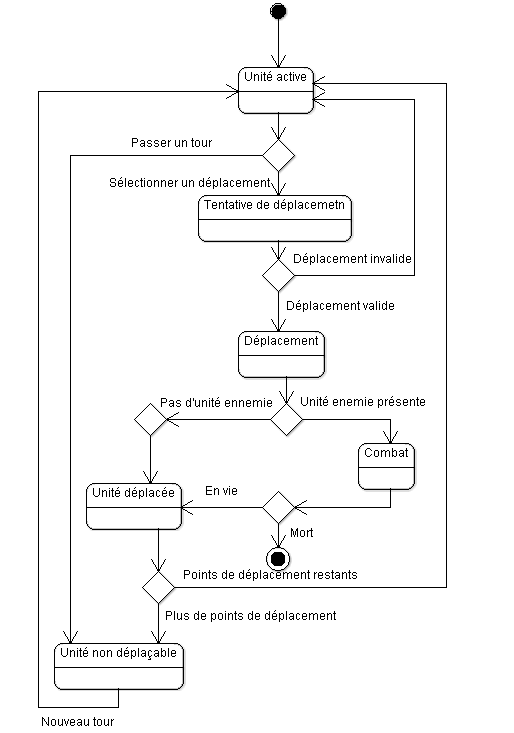
\includegraphics[width=.7\textwidth]{Parties/Images/CycleVieUnite.png}
\caption{Diagramme d'états-transitions : cycle de vie d'une unité}
\label{fig:CycleVieUnite}
\end{figure}

\begin{figure}[!h]
\centering
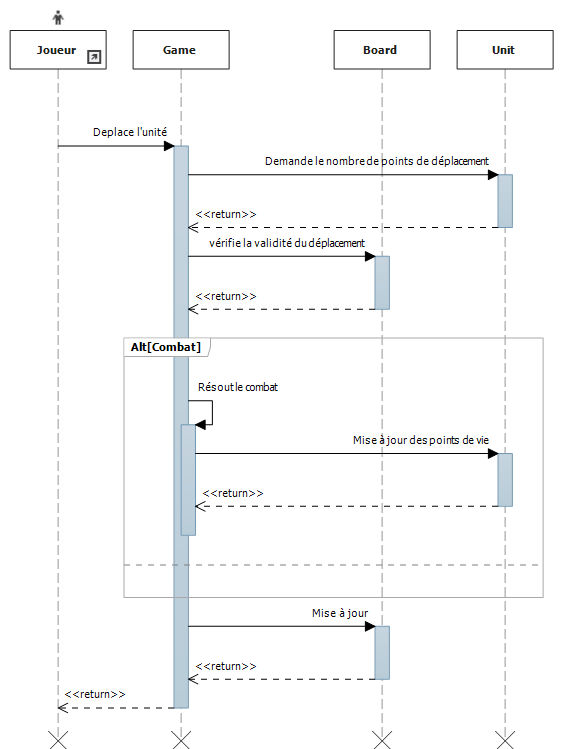
\includegraphics[width=\textwidth]{Parties/Images/seq_DeplacementUnite.png}
\caption{Diagramme de séquence : déplacement d'une unité}
\label{fig:seq_DeplacementUnite}
\end{figure}
